\section{Exceptions}
\label{sec:exceptions}
Exceptions are handled by raising a flag, the offending (or interrupted) instruction address + 1 is stored in an L register.
When an exception condition is detected, the PC is loaded with the indexed special address $idx$ (exception identification immediate).
Reset is treated just as another source of exception.
Being the CR 32 bits wide, the architecture provides a space of 32 different
sources of exceptions, so the first 32 instruction addresses (from 0x00000000 to 0x0000007C) are reserved for exception handlers.\\
Exceptions should only be handled if the correspondig bit in MR is unset. As stated in section \ref{sec:registers}, MR has 33 physical
bits. The higher bit is a global mask for all exceptions and it is a hardware mechanism to avoid nested exceptions
when they are disabled.\\
Interrupts are handled as exceptions. Instructions stored at the special addresses must provide the handling for the exceptions.
Priorities are fixed and they correspond with the order stated in the listing below. Lower ordered exceptions always have higher priority over other
sources of exceptions.\\
The lowest priority is software generated exceptions (\emph{trap} instruction); thus it has the highest number, 31. On the other end, reset has the highest priority
(and the lowest number, 0).\\
The indexed address schema provides space for one instruction to start the handling routine.\\
Sources of exception not defined in this document are left free for future revisions of the architecture or implementation specific
exceptions.

\begin{itemize}
\item E0: Reset
\item E1: System tick.
\item E2: Execute invalid instruction.
\item E3: Misaligned data memory access.
\item E4: Misaligned long GPR access.
\item E5: Misaligned double FPR access.
\item E6: Integer division by zero.
\item E7: Long integer division by zero.
\item E8: Instruction is a FPU operation.
\item E9: Instruction is a FPU extendended operation.
\item E10: FPU\_V flag is set.
\item E11: FPU\_Z flag is set.
\item E12: FPU\_O flag is set.
\item E13: FPU\_U flag is set.
\item E30: Interruption request.
\item E31: Trap.
\end{itemize}

Nested exceptions support is configured by means of the bit 1 of the CFG register. If not supported, the CPU cannot
accept a new source of exception until the handling of the current one has finished. On the other hand, when
nested interruptions are supported, only a higher priority exception can interrupt the current one.\\

\subsection{Exception handling}
\label{ssec:exception_handling}
As stated earlier, the nested exception support can be enabled/disabled through the bit 1 of the CFG register.

\subsubsection{Nested insterruptions disabled}
\label{sssec:nested_irq_disabled}
In table \ref{tbl:nid_steps} interruption handling with nested interruptions disabled is described; pc is the offending (or interrupted) instruction address.

\begin{table}
\begin{center}
\begin{tabu} to \textwidth {|X[r]|X[2,l]|X[l]|X[2,l]|}
\rowfont[c]\bfseries
\hline
Step & Description & Assembly & Registers Status\\
\hline
\hline
1. & Exception $idx$ is raised             &                  & if $(mr[idx]==`0')$ then \\
   &                                       &                  & \hspace{20pt}$l_0[29:0] \leftarrow_{30} (pc + 1)$ \\
   &                                       &                  & \hspace{20pt}$pc \leftarrow_{30} idx$ \\
   &                                       &                  & \hspace{20pt}$mr[32] \leftarrow_{1} 1$ \\
   &                                       &                  & \hspace{20pt}$cr[idx] \leftarrow_{1} 0$ \\
   &                                       &                  & \hspace{20pt}$cfg[0] \leftarrow_{1} 0$ \\
   &                                       &                  & \hspace{20pt}continue with step 2.\\
   &                                       &                  & else\\
   &                                       &                  & \hspace{20pt}Do not handle the exception \\
   &                                       &                  & endif \\
\hline
2. & Jump to the exception handler routine & \texttt{j dis26} & $pc \leftarrow_{30} pc + sx_{30}(dis26)$ \\
\hline
3. & Save context to be used in handler    & User code        & \\
\hline
4. & Handler routine                       & User code        & \\
\hline
5. & Recover context                       & User code        & \\
\hline
6. & Return from exception                 & \texttt{rfe}     & $pc \leftarrow_{30} l_0[29:0]$ \\
   &                                       &                  & $mr[32] \leftarrow_{1} 0$ \\
   &                                       &                  & $cfg[0] \leftarrow_{1} 1$ \\
\hline
\end{tabu}
\end{center}
\caption{Nested Interruptions Disabled Interrupt Sequence}
\label{tbl:nid_steps}
\end{table}


\subsubsection{Nested insterruptions enabled}
\label{sssec:nested_irq_enabled}
In table \ref{tbl:nie_steps} interruption handling with nested interruptions disabled is described; pc is the offending (or interrupted) instruction address.

\begin{table}
\begin{center}
\begin{tabu} to \textwidth {|X[r]|X[2,l]|X[l]|X[2,l]|}
\rowfont[c]\bfseries
\hline
Step & Description & Assembly & Registers Status\\
\hline
\hline
1. & Exception $idx$ is raised             &                  & if $(mr[idx]==`0')$ \&\& $(idx < l_{esp}[35:30])$ then \\
   &                                       &                  & \hspace{20pt}$l_{esp}[29:0] \leftarrow_{30} (pc + 1)$ \\
   &                                       &                  & \hspace{20pt}$esp \leftarrow_{5} (esp + 1)$ \\
   &                                       &                  & \hspace{20pt}$l_{esp}[34:30] \leftarrow_{5} idx$ \\
   &                                       &                  & \hspace{20pt}$pc \leftarrow_{30} idx$ \\
   &                                       &                  & \hspace{20pt}$cr[idx] \leftarrow_{1} 0$ \\
   &                                       &                  & \hspace{20pt}$cfg[0] \leftarrow_{1} 0$ \\
   &                                       &                  & \hspace{20pt}continue with step 2.\\
   &                                       &                  & else\\
   &                                       &                  & \hspace{20pt}Do not handle the exception \\
   &                                       &                  & endif \\
\hline
2. & Jump to the exception handler routine & \texttt{j dis26} & $pc \leftarrow_{30} pc + sx_{30}(dis26)$ \\
\hline
3. & Save context to be used in handler    & User code        & \\
\hline
4. & Handler routine                       & User code        & \\
\hline
5. & Recover context                       & User code        & \\
\hline
6. & Return from exception                 & \texttt{rfe}     & $esp \leftarrow_{5} esp - 1$ \\
   &                                       &                  & $pc \leftarrow_{30} l_{esp}[29:0]$ \\
   &                                       &                  & $cfg[0] \leftarrow_{1} 1$ \\

\hline
\end{tabu}
\end{center}
\caption{Nested Interruptions Enabled Sequence Detail}
\label{tbl:nie_steps}
\end{table}

\subsection{Reset exception}
\label{ssec:reset_exception}
As stated before, reset is just another exception, but there are a few differences with the other sources.\\
The reset exception cannot be masked: altough MR can be written with the lower bit set, the reset exception will not be masked. Also,
it will not be masked by the global mask bit, enabling the reset to happen even if an exception is being handled.\\

\subsubsection{Getting out of the reset exception and booting}
The reset mechanism will set all registers with zero (except L0), though, the first instruction
excecuted by the microprocesor is in address \texttt{0x00000000}, and as the CFG register is zeroed, the microprocesor will run in supervisor mode.
Thus, the reset address is the vectored address for the reset exception. That instruction should be a jump to the reset exception handler. This
handler should implement all the boot code necessary to set up the environment. As L0[29:0] is loaded with 0 (as a consequence of
the reset) the code cannot call $rfe$ to get out of the exception (calling $rfe$ will load the PC with the reset address again). So CFG
register must be manually set to user mode once initialization is done and everything is ready to start running user code via
a \emph{movi2s} instruction.

\subsection{System tick}
\label{ssec:sys_tick}
System tick is a periodic exception internally generated by the CPU hardware.The system timer is a 32 bits down counter that
generates the systick exception when reaches zero. The reload value of the system timer can be configured trough
the STP register.

The CFG register (bit 2) sets the system timer behavior. If unset, the timer will be in free running mode, meaning that
once the timer reaches zero, it will be automatically reloaded with the value $(1024*STP) + 1023$ and will continue counting down.
On the other hand, if set, the system timer will stop when reaches zero and will reload the value $(1024*STP) + 1023$ and
resume the count down after CFG[3] is written with \emph{movi2s}.

The bit 3 of the CFG register is not persistent, it means that goes back to '0' one clock cycle after it was written.
Always returns '0' on read.

\subsection{Interruptions}
The CPU is hardware interrupted by rising the interrupt input port (\emph{irq}) and exception E30 is launched if not masked.
When the processor attends the interruption exception, the $iack$ output is raised by the processor indicating
that the exception was already handled. The $iack$ output is set low by the CPU when a new interruption request occurs. Fig.
\ref{fig:int_sequence} shows a timing diagram of the interruption sequence.

\begin{figure}
\begin{center}
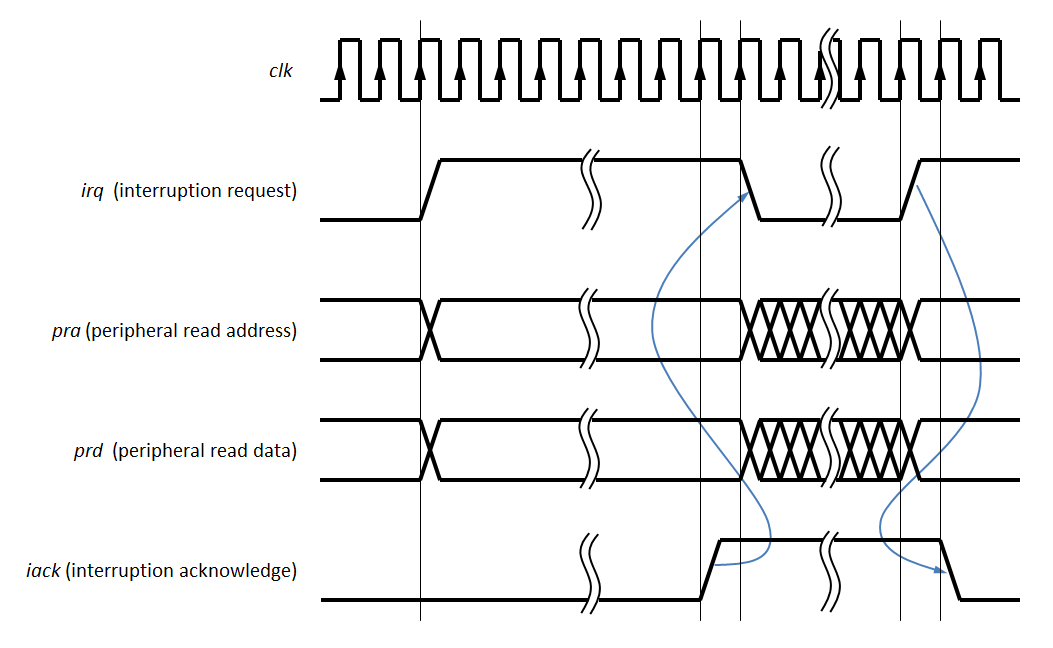
\includegraphics[scale=0.55]{./figures/int_td.png}
\caption{Interruption timing diagram.}
\label{fig:int_sequence}
\end{center}
\end{figure}



